\documentclass[11pt,a4paper]{article}

\usepackage[margin=1in]{geometry}
\usepackage[T1]{fontenc}
\usepackage[utf8]{inputenc}
\usepackage{lmodern}
\usepackage{microtype}
\usepackage{amsmath}
\usepackage{amssymb}
\usepackage{booktabs}
\usepackage{enumitem}
\usepackage{graphicx}
\usepackage{array}
\usepackage{longtable}
\usepackage{float}
\usepackage{hyperref}
\usepackage{tikz}
\usetikzlibrary{arrows.meta, positioning}

\hypersetup{
  colorlinks=true,
  linkcolor=blue,
  urlcolor=blue,
  citecolor=blue,
  pdftitle={Lung Cancer Classification Using CT-Derived Radiomic and Clinical Features},
  pdfauthor={LabIACD-Project1}
}

\title{Lung Cancer Classification Using CT-Derived Radiomic and Clinical Features}
\author{}
\date{\today}

\begin{document}

\maketitle

\begin{abstract}
This paper investigates lung cancer classification from CT-derived radiomic and clinical features using a classical machine learning workflow. The dataset is derived from the LIDC-IDRI collection and organized into prepared feature tables with different standard-deviation settings. The study combines data verification, preprocessing, feature selection, and model evaluation to predict malignancy-related labels from structured tabular inputs.

The main machine learning approach uses feature selection methods such as recursive feature elimination, tree-based importance, variance thresholding, and Lasso, followed by classification with Random Forest and K-Nearest Neighbors models. The experiments show that model performance depends strongly on the selected feature set, with KNN sweeps identifying different best values of $k$ across runs and feature-selection strategies achieving cross-validation scores in the mid-to-high 0.6 range. A representative KNN evaluation produced class-wise precision of 0.57, 0.79, 0.50, and 0.00, and an overall confusion matrix that shows strong performance on the major classes but weak prediction for one class. The results indicate that classical machine learning is a viable baseline for the task, but class imbalance, missing data, and limited representation of some classes remain important constraints.
\end{abstract}

\section{Introduction}


Lung cancer remains one of the leading causes of cancer mortality worldwide, and early diagnosis is critical for improving patient outcomes. CT imaging plays a central role in detection and follow-up because it can reveal nodule characteristics that are not easily captured by routine clinical examination. However, interpretation of CT scans is challenging, especially when nodules are subtle, heterogeneous, or ambiguous across radiologists.

Machine learning provides a practical way to support medical imaging analysis by learning predictive patterns from radiomic descriptors and structured clinical annotations. In this project, the goal is not to replace clinical judgment, but to investigate whether a classical machine learning pipeline can learn useful patterns from the LIDC-IDRI-derived feature tables and provide a reproducible benchmark for later work.

The objectives of the project are:
\begin{enumerate}[leftmargin=*]
    \item Build a clean and reproducible lung cancer classification workflow.
    \item Compare multiple feature selection strategies on the prepared CT feature tables.
    \item Evaluate classical machine learning models using standard classification metrics.
    \item Document the results in a form that can be extended to deeper models or image-based approaches later.
\end{enumerate}

The scope of the work is limited to structured tabular features extracted from CT-related metadata and radiomic summaries. Raw image segmentation, deep convolutional learning, and clinical deployment are outside the present scope.

The paper is organized as follows: Section~2 defines the classification problem. Section~3 reviews related work. Section~4 describes the dataset and its preparation. Section~5 explains the methodology. Section~6 details the experimental setup. Section~7 defines the evaluation metrics. Section~8 presents the results. Section~9 discusses the findings. Section~10 covers limitations. Section~11 addresses ethical considerations. Section~12 proposes future work. Section~13 concludes the paper.

\section{Problem Statement}


This project addresses a multi-class classification problem where the objective is to predict malignancy-related labels from CT-derived tabular features. The input consists of structured radiomic measurements and nodule-level diagnostic fields. The target variable is the malignancy label used throughout the notebooks.

The expected output is a predicted class for each sample, together with class probabilities or confidence scores where supported by the model. The problem is difficult for several reasons: the data contains missing values, some feature groups are redundant, the classes are not uniformly represented, and nodule-level labels may be ambiguous or incomplete. In addition, different feature-selection strategies produce different feature subsets, so model behavior can vary depending on how the input space is reduced.

\section{Related Work}


Lung cancer prediction with machine learning has been studied using both image-based and tabular radiomics workflows. Radiomics-based approaches are particularly attractive because they transform medical images into numerical descriptors that can be used with classical classifiers. This often reduces computational cost compared with end-to-end deep learning and improves interpretability for small to medium-sized datasets.

Deep learning methods, especially CNNs, have shown strong performance when trained on large image corpora, but they typically require more data, more compute, and more extensive validation. Classical machine learning remains important in medical research because it is easier to inspect, faster to train, and often more suitable when the available data is limited or already represented as features.

The LIDC-IDRI dataset is a common benchmark in this area because it combines CT scans, nodule annotations, and malignancy-related labels. Prior work on this dataset has used both handcrafted radiomic features and deep networks. The approach chosen here is motivated by the project structure and the available prepared feature tables: the data is already tabular, so a classical machine learning pipeline is a natural and reproducible starting point.

\section{Dataset}
\subsection{Dataset Description}


The project uses data derived from the LIDC-IDRI collection hosted by the Cancer Imaging Archive (TCIA). LIDC-IDRI contains thoracic CT scans with lesion annotations contributed by multiple radiologists. The repository includes prepared feature tables named \texttt{data\_0.5.csv}, \texttt{data\_1.0.csv}, and \texttt{data\_1.5.csv}, along with source metadata under \texttt{data/}.

The target variable used in the notebooks is the malignancy label. The feature tables contain radiomic and diagnostic descriptors extracted from CT nodules and related metadata fields.

The exact number of samples and features depends on the table and preprocessing stage. Based on the notebook outputs, the data is large enough to support multiple feature-selection experiments, but not so large that classical models become impractical.

\subsection{Data Preparation}


Initial inspection focused on identifier consistency, duplicates, whitespace issues, and missing values. The verification notebook checks ID formatting, duplicate IDs, cross-table consistency, and missing data patterns.

Missing values are concentrated in several diagnostic fields, including nodule-level diagnosis and diagnosis method columns. The notebooks also show that some feature columns are entirely zero-valued, which indicates either absent information or encoded unknowns. This makes careful preprocessing necessary before modeling.

The class distribution is not perfectly balanced, and this is visible in the classification results, where one class is not predicted at all in a representative run. That imbalance affects precision, recall, and confusion-matrix behavior.

\section{Methodology}
\subsection{Overall Pipeline}


The workflow is summarized in Figure~\ref{fig:workflow}:

\begin{figure}[H]
\centering
\resizebox{0.98\linewidth}{!}{%
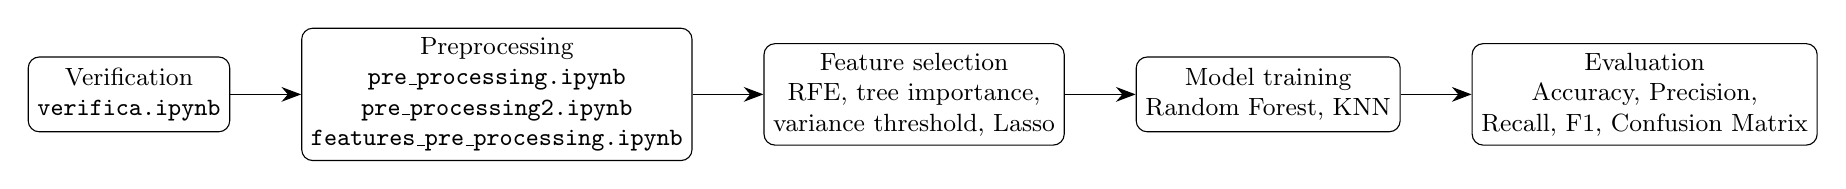
\begin{tikzpicture}[
    node distance=0.9cm,
    every node/.style={draw, rounded corners, align=center, font=\small, minimum width=2.3cm, minimum height=0.95cm},
    >={Stealth[length=2.5mm]}
]
    \node (a) {Verification\\\texttt{verifica.ipynb}};
    \node (b) [right=of a] {Preprocessing\\\texttt{pre\_processing.ipynb}\\\texttt{pre\_processing2.ipynb}\\\texttt{features\_pre\_processing.ipynb}};
    \node (c) [right=of b] {Feature selection\\RFE, tree importance,\\variance threshold, Lasso};
    \node (d) [right=of c] {Model training\\Random Forest, KNN};
    \node (e) [right=of d] {Evaluation\\Accuracy, Precision,\\Recall, F1, Confusion Matrix};

    \draw[->] (a) -- (b);
    \draw[->] (b) -- (c);
    \draw[->] (c) -- (d);
    \draw[->] (d) -- (e);
\end{tikzpicture}%
}
\caption{Notebook-based workflow used in the project.}
\label{fig:workflow}
\end{figure}

The workflow has five main stages: data verification, preprocessing, feature engineering, feature selection, and model training/evaluation.

\subsection{Data Preprocessing}
Preprocessing includes loading the prepared CSV files, harmonizing column names, inspecting missing values, and cleaning diagnostic fields. Because the notebooks are organized into separate stages, the preprocessing notebooks are used as dependencies for later feature-selection and modeling notebooks.

The current workflow performs data validation and cleaning rather than heavy outlier engineering. Missing values are inspected and reported, and the feature tables are normalized into a reusable tabular format. Some columns are filtered or interpreted as unknown/zero-valued entries.

\subsection{Feature Engineering}
Feature engineering in this project is mostly driven by the existing radiomic and clinical descriptors in the prepared tables. The notebooks perform label handling and column standardization rather than generating large numbers of new synthetic variables.

Feature encoding is handled through preprocessing of diagnosis labels and consistent column naming. Feature scaling is not emphasized in the current notebook workflow because the primary models include tree-based methods, although scaled features would be useful for future distance-based or neural approaches.

\subsection{Feature Selection}
Four main selection strategies are used:
\begin{enumerate}[leftmargin=*]
    \item Recursive Feature Elimination with cross-validation (RFECV) using Random Forest.
    \item Tree-based feature importance with thresholds of 0.01 and 0.02.
    \item Variance threshold filtering.
    \item Lasso-based sparse selection.
\end{enumerate}

These methods were selected because they provide complementary views of feature relevance: recursive elimination searches for a performant subset, tree importance identifies strong nonlinear predictors, variance threshold removes low-information features, and Lasso keeps only features with non-zero linear contribution.

The notebooks show that the best cross-validation scores occur in the mid-to-high 0.6 range depending on the feature set. Tree-based and Lasso-based subsets were among the strongest performers in the comparison plot.

\subsection{Machine Learning Models}
\subsubsection{Random Forest}


Random Forest is used as the main classifier for feature selection and evaluation because it handles nonlinear relationships, is robust to mixed feature types, and provides feature importance estimates.

\begin{itemize}[leftmargin=*]
    \item \textbf{Advantages:} Works well on tabular data; supports feature importance analysis; handles nonlinear interactions.
    \item \textbf{Limitations:} Can be less interpretable than simpler linear models; sensitive to class imbalance if not tuned; may overfit if feature selection is weak.
\end{itemize}

\subsubsection{K-Nearest Neighbors}


KNN is used as a comparison model and as a small hyperparameter sweep over $k$. It provides a simple baseline and helps illustrate how local similarity behaves on the prepared feature tables.

\begin{itemize}[leftmargin=*]
    \item \textbf{Advantages:} Simple and intuitive; useful baseline for tabular similarity structure.
    \item \textbf{Limitations:} Sensitive to scaling and irrelevant features; can degrade quickly in high dimensions; computational cost grows with the training set.
\end{itemize}

\section{Experimental Setup}
\subsection{Development Environment}


The project is implemented in Python and organized in Jupyter notebooks. The main libraries used are pandas, NumPy, matplotlib, seaborn, and scikit-learn. The repository currently documents Python package dependencies in \texttt{requirements.txt}.

Hardware details are not recorded in the notebook outputs, so the exact machine specification is not reported here.

\subsection{Training Procedure}


\begin{itemize}
    \item The notebooks use a train/test split with \texttt{test\_size=0.2} and \texttt{random\_state=42}.
    \item Cross-validation uses stratified folds to preserve class proportions during evaluation.
    \item Random Forest models are commonly initialized with \texttt{random\_state=42} for reproducibility, and KNN is evaluated over several values of $k$.
    \item Random Forest remains the core estimator for feature selection and comparison.
\end{itemize}

\subsection{Evaluation Strategy}


The evaluation protocol compares multiple feature sets under the same classification setting. Performance is measured with cross-validation and held-out test results where available. This makes it possible to compare feature-selection methods on a common basis.

Reproducibility is supported by fixed random seeds, notebook-based execution, and explicit dependency listing. The notebooks are organized so that the preprocessing dependencies can be loaded from later stages.

\section{Evaluation Metrics}


The project uses the following metrics:
\begin{itemize}[leftmargin=*]
    \item Accuracy: overall proportion of correct predictions.
    \item Precision: how many predicted positives are correct.
    \item Recall: how many true positives are recovered.
    \item F1-score: harmonic mean of precision and recall.
    \item ROC-AUC: useful for ranking quality when probability estimates are available.
    \item Confusion matrix: shows class-by-class mistakes and reveals failure modes.
\end{itemize}

These metrics were chosen because medical classification problems require more than a single accuracy number. In particular, precision and recall are important when a minority class is clinically meaningful, and the confusion matrix helps identify whether the model is collapsing into majority-class predictions.

\section{Results}
\subsection{Model Performance}


The notebook experiments show that performance varies with the selected feature set. KNN sweeps identified different best values of $k$ across runs, including $k = 4$ and $k = 6$ in separate comparisons. This indicates that the local neighborhood structure of the data changes materially with the underlying feature subset.

Feature-selection experiments produced the strongest cross-validation scores in the mid-to-high 0.6 range. Tree-based and Lasso-based subsets were especially competitive, while RFE remained stable across the three prepared data tables.

\subsection{Feature Importance}


The most relevant features depend on the selection strategy. RFE returns compact subsets tailored to the classifier objective, tree-based importance highlights features with high nonlinear predictive value, and Lasso keeps sparse linear predictors. The comparison suggests that no single feature subset dominates all criteria, but tree-based and sparse selections give the best overall balance in the notebook runs.

\subsection{Visual Results}


The repository includes exported figures from the notebook outputs, including KNN performance sweeps, confusion matrices, and feature-selection comparison plots. Figure~\ref{fig:knn-sweep} shows the KNN sweep, Figure~\ref{fig:confusion-matrix} shows the confusion matrix, Figure~\ref{fig:confusion-matrix-values} shows the annotated confusion matrix, Figure~\ref{fig:pairplot} shows the pairplot, and Figure~\ref{fig:feature-comparison} shows the feature-selection comparison.

\begin{figure}[H]
\centering
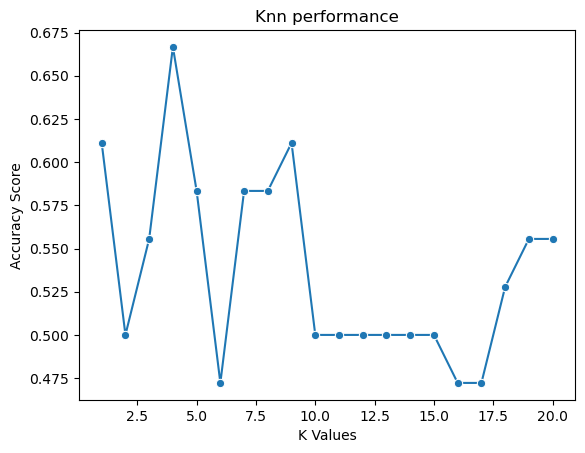
\includegraphics[width=0.95\linewidth]{figures/trainingmodels_01.png}
\caption{KNN performance sweep.}
\label{fig:knn-sweep}
\end{figure}

\begin{figure}[H]
\centering
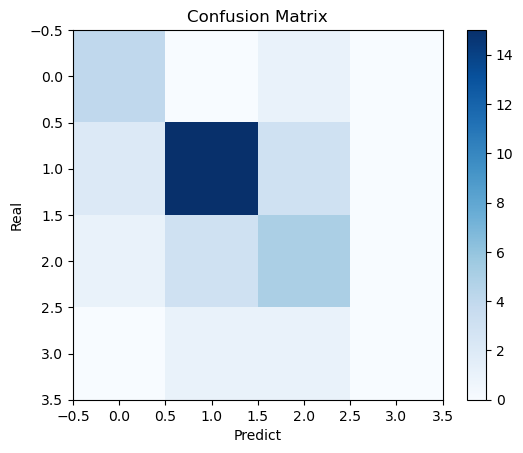
\includegraphics[width=0.95\linewidth]{figures/trainingmodels_02.png}
\caption{Confusion matrix.}
\label{fig:confusion-matrix}
\end{figure}

\begin{figure}[H]
\centering
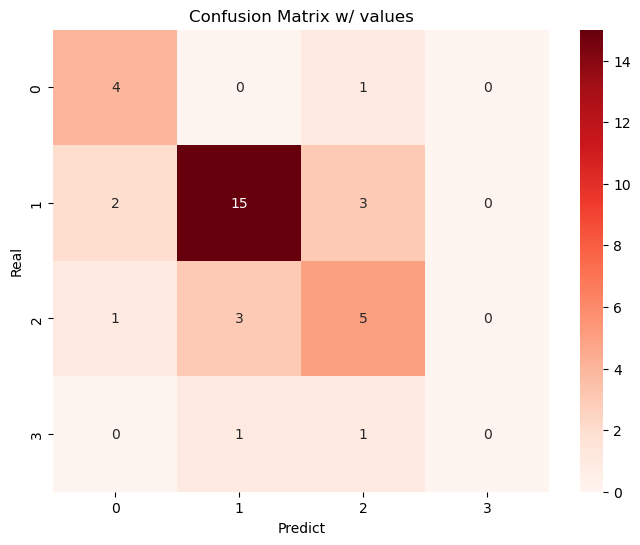
\includegraphics[width=0.95\linewidth]{figures/trainingmodels_03.png}
\caption{Confusion matrix with values.}
\label{fig:confusion-matrix-values}
\end{figure}

\begin{figure}[H]
\centering
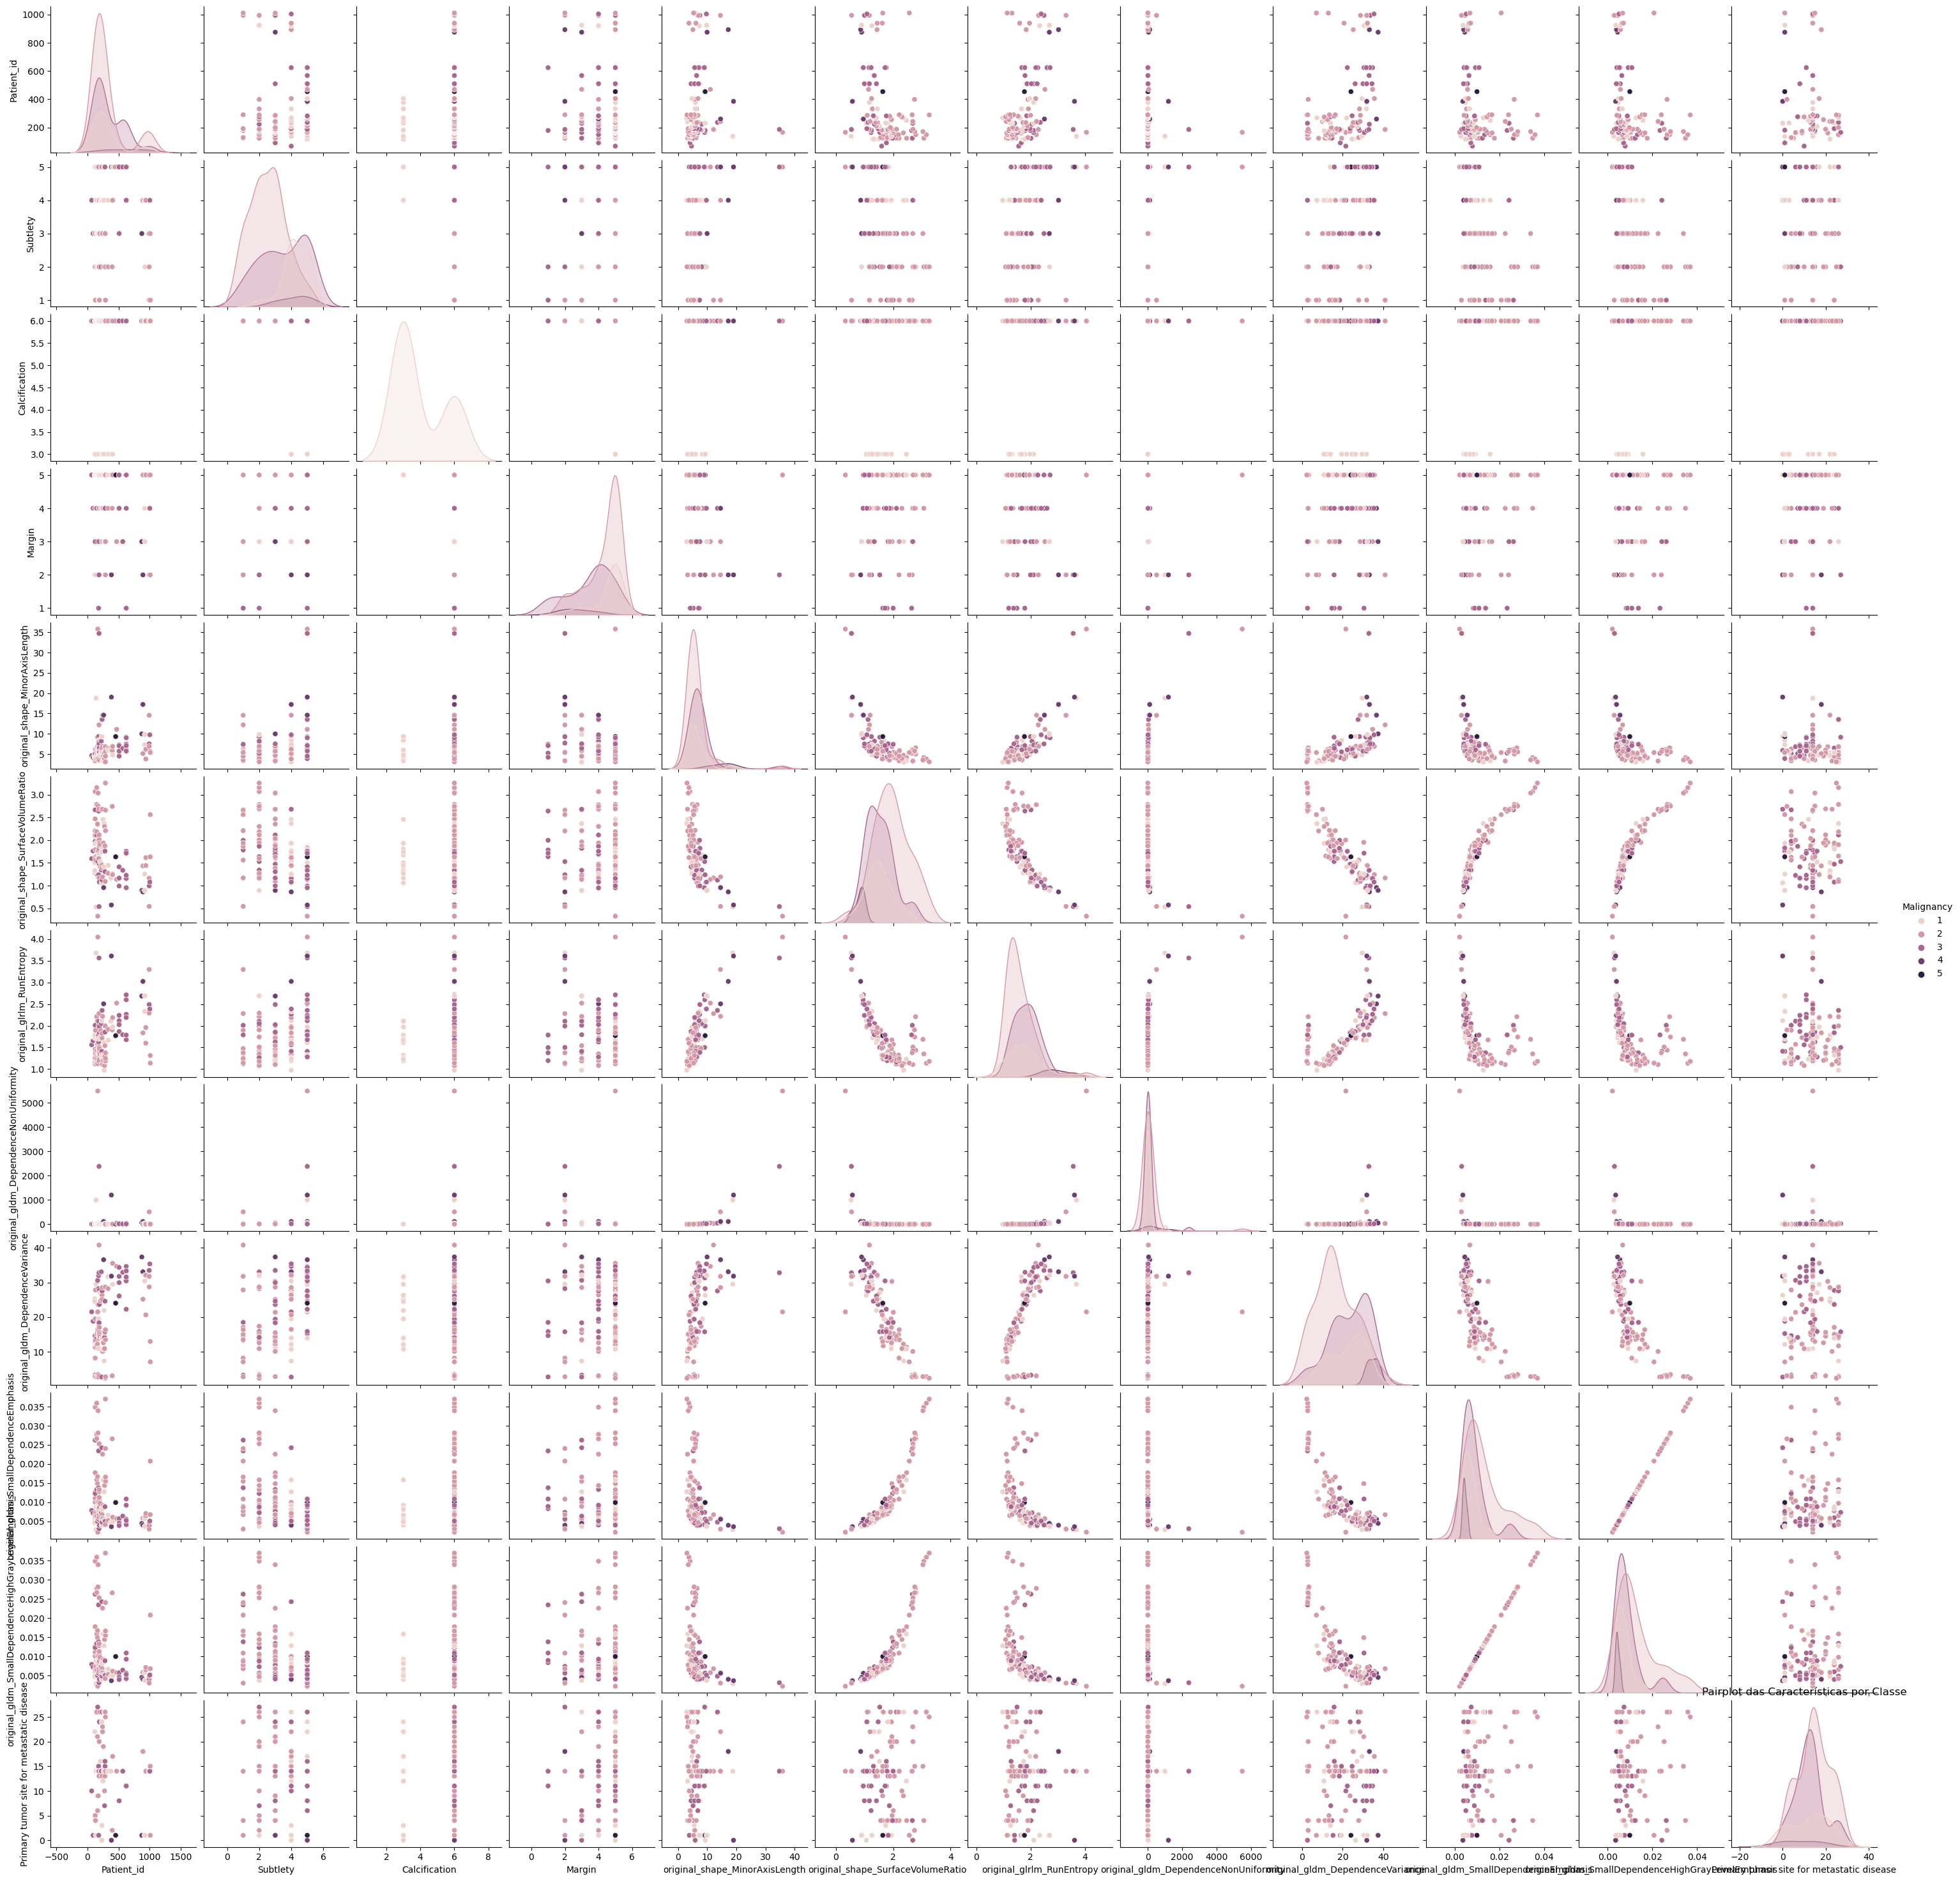
\includegraphics[width=0.95\linewidth]{figures/trainingmodels_04.png}
\caption{Pairplot of selected features.}
\label{fig:pairplot}
\end{figure}

\begin{figure}[H]
\centering
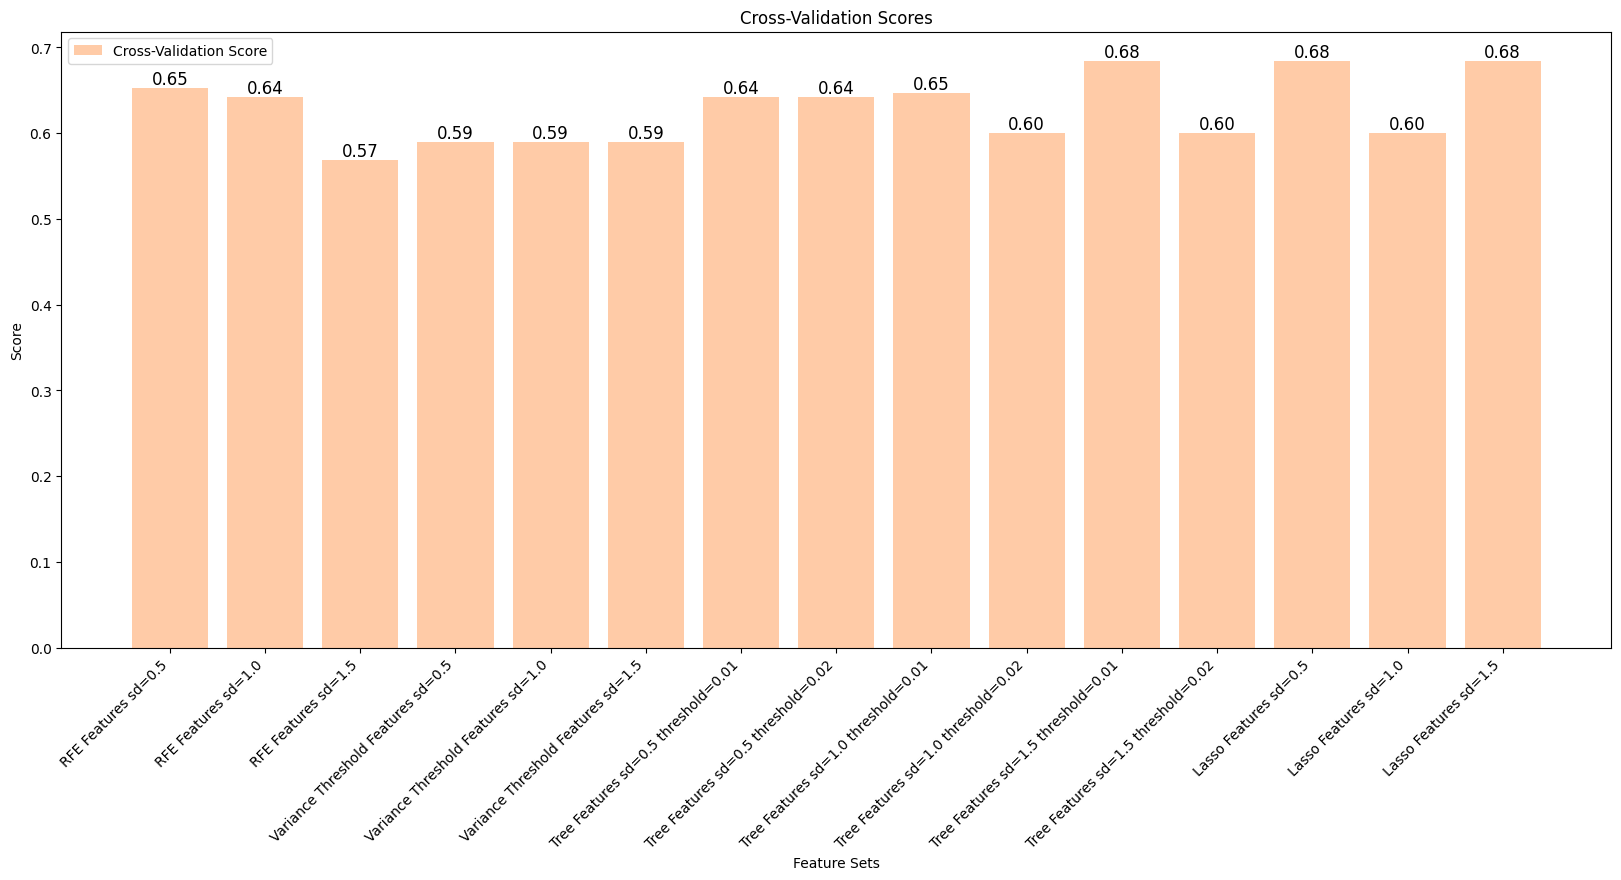
\includegraphics[width=0.95\linewidth]{figures/feature_selection_01.png}
\caption{Feature selection comparison.}
\label{fig:feature-comparison}
\end{figure}

Table~\ref{tab:confusion-matrix} summarizes a representative KNN evaluation.

\begin{table}[H]
\centering
\begin{tabular}{lrrrr}
\toprule
 & Pred 0 & Pred 1 & Pred 2 & Pred 3 \\
\midrule
Real 0 & 4 & 0 & 1 & 0 \\
Real 1 & 2 & 15 & 3 & 0 \\
Real 2 & 1 & 3 & 5 & 0 \\
Real 3 & 0 & 1 & 1 & 0 \\
\bottomrule
\end{tabular}
\caption{Representative confusion matrix from the notebook evaluation.}
\label{tab:confusion-matrix}
\end{table}

Table~\ref{tab:class-scores} shows the same run's class-wise scores.

\begin{table}[H]
\centering
\begin{tabular}{lrrrr}
\toprule
Metric & Class 0 & Class 1 & Class 2 & Class 3 \\
\midrule
Precision & 0.57 & 0.79 & 0.50 & 0.00 \\
Recall & 0.80 & 0.75 & 0.56 & 0.00 \\
F1-score & 0.67 & 0.77 & 0.53 & 0.00 \\
\bottomrule
\end{tabular}
\caption{Representative class-wise scores from the notebook evaluation.}
\label{tab:class-scores}
\end{table}

\subsection{Model Comparison}


Random Forest appears to be the most useful model family in the current project because it supports both feature selection and classification, and it performs consistently across the prepared feature subsets. KNN is useful as a comparator, but its performance is more sensitive to feature-set choice and dimensionality.

From a computational perspective, the pipeline is lightweight enough to run interactively in notebooks. The main cost comes from cross-validation and repeated training across feature sets.

\section{Discussion}


The results suggest that preprocessing and feature selection have a substantial impact on performance. When feature sets are reduced using tree importance or Lasso, the classifier often performs competitively or better than with less selective subsets. This supports the idea that the dataset contains redundant and weakly informative variables that can be removed without losing useful signal.

The difference between feature-selection strategies is also informative. RFE is objective-driven and tends to preserve model performance, while tree-based methods can surface nonlinear signals that are missed by simple variance filters. Lasso is more aggressive and can produce compact subsets that are easier to inspect, but it may discard features that matter in nonlinear interactions.

The representative confusion matrix shows that the model is good at identifying the majority classes but struggles with one class entirely. This is consistent with class imbalance and suggests that future work should focus on balancing techniques, threshold tuning, and external validation.

\section{Limitations}


The current study has several limitations:
\begin{itemize}[leftmargin=*]
    \item The dataset is tabular and derived from prepared feature tables rather than raw images.
    \item Some classes are underrepresented, which affects minority-class recall.
    \item Missing values are frequent in the diagnostic fields.
    \item The project currently uses classical machine learning rather than end-to-end image learning.
    \item Hardware and execution environment details are not fully recorded in the notebooks.
    \item The model evaluation is internal to the prepared tables and does not yet include external clinical validation.
\end{itemize}


\section{Ethical Considerations}


This project works with anonymized medical imaging data and should be treated as a decision-support experiment rather than a clinical diagnostic tool. Patient privacy depends on the anonymization provided by the source dataset, and any downstream reuse should preserve that anonymization.

Explainability is important in medical AI, so classical models and feature selection are useful because they expose which variables contribute to the decision process. Fairness and bias remain concerns, especially if the underlying cohort is not representative of the broader population.

The system should not be interpreted as a standalone clinical decision engine. Any real-world use would require medical oversight, regulatory review, and strict validation. If future deployment is considered, privacy and compliance requirements such as GDPR or the EU AI Act, where applicable, should be assessed.

\section{Future Work}


Several extensions are natural next steps:
\begin{itemize}[leftmargin=*]
    \item Train deep learning models such as CNNs directly on raw CT images.
    \item Add explainable AI methods such as SHAP or LIME.
    \item Validate the pipeline on an external dataset.
    \item Perform more systematic hyperparameter optimization.
    \item Explore ensemble learning across multiple feature-selection strategies.
    \item Investigate federated learning for privacy-preserving multi-site analysis.
    \item Document deployment constraints and clinical integration requirements.
\end{itemize}


\section{Conclusion}


This project demonstrates a reproducible classical machine learning workflow for lung cancer classification from CT-derived features. The method combines verification, preprocessing, feature selection, and model evaluation on prepared LIDC-IDRI-derived tables. The experiments show that feature selection materially affects performance and that Random Forest-based approaches are particularly useful for this type of tabular medical data.

The main contribution of the project is a clean baseline pipeline that can be reused and extended. The work shows that classical methods can produce meaningful results on structured CT features, but also highlights the importance of class balance, data quality, and careful validation.


\section{References}


\begin{enumerate}[leftmargin=*]
    \item The Cancer Imaging Archive (TCIA). LIDC-IDRI dataset.
    \item Kumar et al., radiomics and lung nodule classification literature.
    \item scikit-learn documentation.
    \item pandas documentation.
    \item NumPy documentation.
    \item matplotlib documentation.
    \item seaborn documentation.
\end{enumerate}

\appendix
\section{Repository Structure}
\begin{verbatim}
repository-root/
|-- data/
|   |-- MetaData.csv
|   \-- primary.text
|-- data_0.5.csv
|-- data_1.0.csv
|-- data_1.5.csv
|-- figures/
|-- notebooks/
|   |-- 00_verification/
|   |   \-- verifica.ipynb
|   |-- 01_preprocessing/
|   |   |-- pre_processing.ipynb
|   |   |-- pre_processing2.ipynb
|   |   \-- features_pre_processing.ipynb
|   |-- 02_feature_selection/
|   |   \-- feature_selection.ipynb
|   \-- 03_modeling/
|       \-- trainingmodels.ipynb
|-- README.md
|-- requirements.txt
\-- TECHNICAL_PAPER.md
\end{verbatim}

\section{Reproducibility}
\subsection{Installation}
\begin{verbatim}
pip install -r requirements.txt
\end{verbatim}

\subsection{Dataset Download Instructions}
The repository already includes the prepared CSV files used in the notebooks. If you need the raw source data, retrieve it from TCIA and regenerate the prepared tables using the preprocessing notebooks.

\subsection{How to Execute the Pipeline}
\begin{enumerate}[leftmargin=*]
    \item Open the notebooks in the \texttt{notebooks/} folder.
    \item Run \texttt{notebooks/00\_verification/verifica.ipynb} first.
    \item Run the preprocessing notebooks in \texttt{notebooks/01\_preprocessing/}.
    \item Run \texttt{notebooks/02\_feature\_selection/feature\_selection.ipynb}.
    \item Run \texttt{notebooks/03\_modeling/trainingmodels.ipynb}.
\end{enumerate}

\subsection{Expected Outputs}
\begin{itemize}[leftmargin=*]
    \item Data quality and missing-value reports.
    \item Selected feature subsets for RFE, tree importance, variance threshold, and Lasso.
    \item Cross-validation score comparison plots.
    \item Confusion matrices and class-wise metrics.
    \item Exported figures in the \texttt{figures/} folder.
\end{itemize}

\end{document}
